\documentclass[tikz,border=4pt]{standalone}
\usetikzlibrary{calc}

\begin{document}
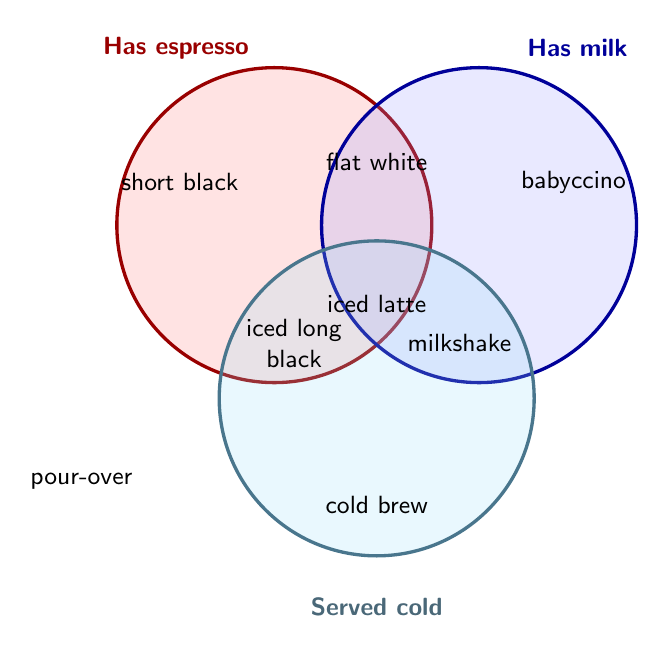
\begin{tikzpicture}[
  font=\sffamily\small,
  set/.style={line width=1.2pt, fill opacity=0.22},
  drink/.style={align=center, inner sep=1pt},
  setlabel/.style={font=\sffamily\bfseries\small, align=center}
]

% ---- the three sets ----
\draw[set, draw=red!60!black,  fill=red!50]    (-1.3, 0.8) circle (2cm); % Has espresso
\draw[set, draw=blue!60!black, fill=blue!40]   ( 1.3, 0.8) circle (2cm); % Has milk
\draw[set, draw=cyan!50!black, fill=cyan!40]   ( 0.0,-1.4) circle (2cm); % Served cold

% ---- set labels ----
\node[setlabel, text=red!60!black]  at (-2.55, 3.05) {Has espresso};
\node[setlabel, text=blue!60!black] at ( 2.55, 3.05) {Has milk};
\node[setlabel, text=cyan!40!black] at ( 0.0, -4.05){Served cold};

% ---- drinks in their regions ----
% espresso only (hot, no milk): short black
\node[drink] at (-2.5, 1.35) {short black};
% milk only (no espresso, warm): babyccino
\node[drink] at ( 2.5, 1.35) {babyccino};
% cold only (no espresso, no milk): cold brew
\node[drink] at ( 0.0,-2.75) {cold brew};
% espresso + milk (hot): flat white
\node[drink] at ( 0.0, 1.60) {flat white};
% espresso + cold (no milk): iced long black
\node[drink] at (-1.05,-0.70) {iced long\\black};
% milk + cold (no espresso): milkshake
\node[drink] at ( 1.05,-0.70) {milkshake};
% all three: iced latte
\node[drink] at ( 0.0,-0.20) {iced latte};
% none of the three (filter coffee, hot, no milk): pour-over
\node[drink] at (-3.75,-2.45) {pour-over};

\end{tikzpicture}
\end{document}
